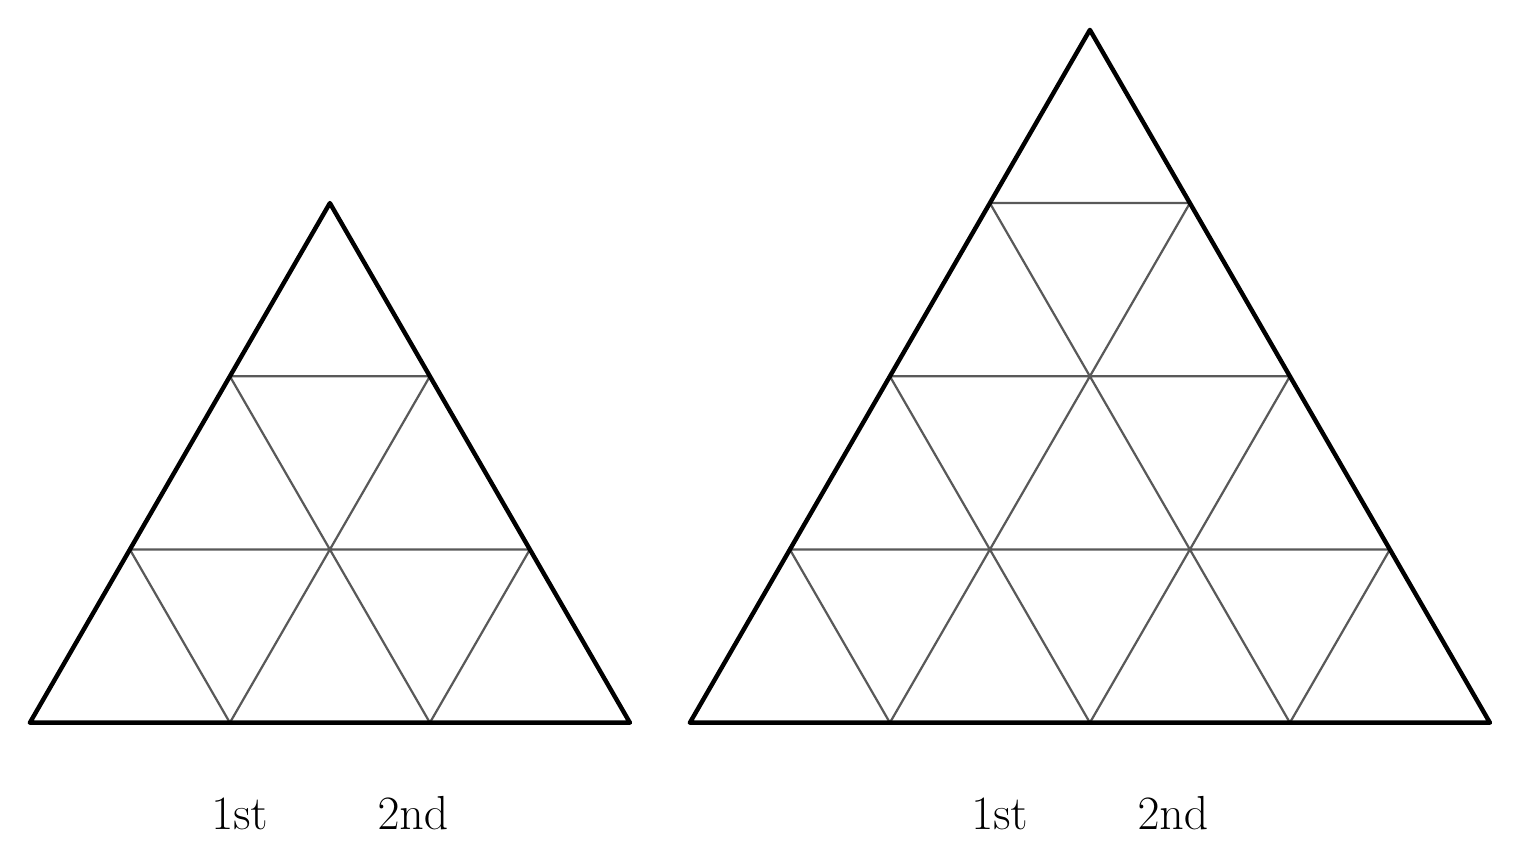
\begin{tikzpicture}[x=1in,y=1in]
\draw[line width=0.8pt, black!65] (1.65,1.316) -- (2.15,0.45) (1.15,0.45) -- (1.65,1.316) (1.15,0.45) -- (0.65,1.316) (0.65,1.316) -- (1.65,1.316) (1.15,2.1821) -- (2.15,2.1821) (1.65,1.316) -- (2.65,1.316) (2.15,0.45) -- (2.65,1.316) (1.65,1.316) -- (1.15,2.1821) (1.65,1.316) -- (2.15,2.1821);
\draw[line width=1.6pt, black, line join=round] (3.15,0.45) -- (1.65,3.0481) -- (0.15,0.45) -- cycle;
\node[anchor=center, inner sep=0pt] at (1.65,0) {\LARGE 1st\hspace{0.55in}2nd};
\draw[line width=0.8pt, black!65] (4.45,0.45) -- (3.95,1.316) (3.95,1.316) -- (4.95,1.316) (4.45,0.45) -- (4.95,1.316) (4.45,2.1821) -- (5.45,2.1821) (5.45,2.1821) -- (4.95,3.0481) (4.95,1.316) -- (5.45,0.45) (4.95,1.316) -- (5.95,1.316) (5.45,0.45) -- (5.95,1.316) (5.45,2.1821) -- (6.45,2.1821) (5.45,2.1821) -- (5.95,3.0481) (5.95,1.316) -- (6.45,0.45) (6.95,1.316) -- (5.95,1.316) (6.95,1.316) -- (6.45,0.45) (5.95,1.316) -- (6.45,2.1821) (4.95,1.316) -- (4.45,2.1821) (4.95,1.316) -- (5.45,2.1821) (5.45,2.1821) -- (5.95,1.316) (4.95,3.0481) -- (5.95,3.0481);
\draw[line width=1.6pt, black, line join=round] (3.45,0.45) -- (7.45,0.45) -- (5.45,3.9141) -- cycle;
\node[anchor=center, inner sep=0pt] at (5.45,0) {\LARGE 1st\hspace{0.55in}2nd};
\end{tikzpicture}
